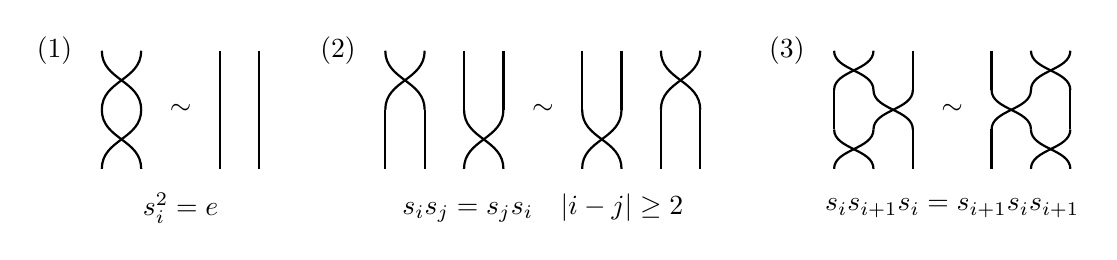
\begin{tikzpicture}
\node at (-0.6,0) {(1)};
\draw[thick] (0.000,0.000) .. controls (0.000,-0.375) and (0.500,-0.375) .. (0.500,-0.750);
\draw[thick] (0.500,0.000) .. controls (0.500,-0.375) and (0.000,-0.375) .. (0.000,-0.750);
\draw[thick] (0.000,-0.750) .. controls (0.000,-1.125) and (0.500,-1.125) .. (0.500,-1.500);
\draw[thick] (0.500,-0.750) .. controls (0.500,-1.125) and (0.000,-1.125) .. (0.000,-1.500);
\node at (1.0,-0.75) {$\sim$};
\draw[thick] (1.500,0.000) -- (1.500,-1.500);
\draw[thick] (2.000,0.000) -- (2.000,-1.500);
\node at (1.0,-2.0) {$s_i^2=e$};
\node at (3.00,0) {(2)};
\draw[thick] (3.600,0.000) .. controls (3.600,-0.375) and (4.100,-0.375) .. (4.100,-0.750);
\draw[thick] (4.100,0.000) .. controls (4.100,-0.375) and (3.600,-0.375) .. (3.600,-0.750);
\draw[thick] (4.600,0.000) -- (4.600,-0.750);
\draw[thick] (5.100,0.000) -- (5.100,-0.750);
\draw[thick] (4.600,-0.750) .. controls (4.600,-1.125) and (5.100,-1.125) .. (5.100,-1.500);
\draw[thick] (5.100,-0.750) .. controls (5.100,-1.125) and (4.600,-1.125) .. (4.600,-1.500);
\draw[thick] (3.600,-0.750) -- (3.600,-1.500);
\draw[thick] (4.100,-0.750) -- (4.100,-1.500);
\node at (5.60,-0.75) {$\sim$};
\draw[thick] (7.100,0.000) .. controls (7.100,-0.375) and (7.600,-0.375) .. (7.600,-0.750);
\draw[thick] (7.600,0.000) .. controls (7.600,-0.375) and (7.100,-0.375) .. (7.100,-0.750);
\draw[thick] (6.100,0.000) -- (6.100,-0.750);
\draw[thick] (6.600,0.000) -- (6.600,-0.750);
\draw[thick] (6.100,-0.750) .. controls (6.100,-1.125) and (6.600,-1.125) .. (6.600,-1.500);
\draw[thick] (6.600,-0.750) .. controls (6.600,-1.125) and (6.100,-1.125) .. (6.100,-1.500);
\draw[thick] (7.100,-0.750) -- (7.100,-1.500);
\draw[thick] (7.600,-0.750) -- (7.600,-1.500);
\node at (5.60,-2.0) {$s_is_j=s_js_i\quad |i-j|\ge 2$};
\node at (8.70,0) {(3)};
\draw[thick] (9.300,0.000) .. controls (9.300,-0.250) and (9.800,-0.250) .. (9.800,-0.500);
\draw[thick] (9.800,0.000) .. controls (9.800,-0.250) and (9.300,-0.250) .. (9.300,-0.500);
\draw[thick] (10.300,0.000) -- (10.300,-0.500);
\draw[thick] (9.800,-0.500) .. controls (9.800,-0.750) and (10.300,-0.750) .. (10.300,-1.000);
\draw[thick] (10.300,-0.500) .. controls (10.300,-0.750) and (9.800,-0.750) .. (9.800,-1.000);
\draw[thick] (9.300,-0.500) -- (9.300,-1.000);
\draw[thick] (9.300,-1.000) .. controls (9.300,-1.250) and (9.800,-1.250) .. (9.800,-1.500);
\draw[thick] (9.800,-1.000) .. controls (9.800,-1.250) and (9.300,-1.250) .. (9.300,-1.500);
\draw[thick] (10.300,-1.000) -- (10.300,-1.500);
\node at (10.80,-0.75) {$\sim$};
\draw[thick] (11.800,0.000) .. controls (11.800,-0.250) and (12.300,-0.250) .. (12.300,-0.500);
\draw[thick] (12.300,0.000) .. controls (12.300,-0.250) and (11.800,-0.250) .. (11.800,-0.500);
\draw[thick] (11.300,0.000) -- (11.300,-0.500);
\draw[thick] (11.300,-0.500) .. controls (11.300,-0.750) and (11.800,-0.750) .. (11.800,-1.000);
\draw[thick] (11.800,-0.500) .. controls (11.800,-0.750) and (11.300,-0.750) .. (11.300,-1.000);
\draw[thick] (12.300,-0.500) -- (12.300,-1.000);
\draw[thick] (11.800,-1.000) .. controls (11.800,-1.250) and (12.300,-1.250) .. (12.300,-1.500);
\draw[thick] (12.300,-1.000) .. controls (12.300,-1.250) and (11.800,-1.250) .. (11.800,-1.500);
\draw[thick] (11.300,-1.000) -- (11.300,-1.500);
\node at (10.80,-2.0) {$s_is_{i+1}s_i=s_{i+1}s_is_{i+1}$};
\end{tikzpicture}
